% Define table for personas.
\newcommand{\persona}[4]{%
    \textbf{#1}
    \small\begin{tabular}[t]{|p{.8in} | p{1.5in}|}
        \hline
        \textbf{Preferences} & #2 \\\hline
        \textbf{Pain Points} & #3 \\\hline
        \textbf{Goals} & #4 \\
        \hline
    \end{tabular}
    \vspace{4pt}
}


\chapter{Introduction}
\label{chap:introduction}

\section{Background}
\label{section:background}

In campus and factory environments, tracking individuals across multiple cameras is essential for security, operational efficiency, and resource management. Security personnel need to monitor suspicious activities, administrators must understand space utilization patterns, and emergency responders require real-time location data during incidents. Without effective tracking, these environments face significant blind spots in their surveillance systems, compromising both safety and operational effectiveness \cite{wangetal:2021}.

When a person moves between camera views, maintaining their consistent identity becomes challenging. Current systems often lose track of individuals as they transition between cameras, creating fragmented surveillance coverage. This problem is particularly acute in large campuses with numerous buildings or factories with complex layouts where dozens of cameras operate independently without sharing identification data.

Environmental factors further complicate tracking efforts. Varying lighting conditions between indoor and outdoor spaces, crowded areas during peak hours, and occlusions from structures or equipment create scenarios where individuals are frequently lost from view. Additionally, the diverse camera placements—some overhead, others at eye level—result in drastically different perspectives of the same person.

The motivation of this project is to develop an integrated multi-camera tracking system that maintains consistent identity recognition across distributed camera networks, enabling seamless surveillance coverage in campus and factory environments. By solving the challenges of cross-camera identity preservation, our solution aims to enhance security monitoring capabilities, improve emergency response times, and provide valuable data for facility management and resource allocation.
\section{Problem Statement}
\label{section:problem-statement}

The problem addressed by the \usevar{\srsTitle} is the technical challenge of maintaining consistent person identification and tracking across multiple non-overlapping camera views in urban environments. When individuals move between camera views in a city, current systems lose track of their identities due to the difficulty of matching appearance features across different perspectives, lighting conditions, occlusions, and the significant temporal and spatial gaps between camera views.

Specifically, the system must solve three interconnected technical problems:

First, the re-identification problem—determining that a person appearing in one camera view is the same individual previously seen in another camera view—requires robust feature extraction that remains consistent despite environmental variations inherent to outdoor urban settings. Current approaches struggle with this matching process, particularly under varying lighting conditions from daylight to nighttime, when viewing individuals from different angles, or when appearance changes due to distance or partial visibility.

Second, the spatial mapping problem involves transforming observations from multiple cameras distributed across city blocks into a coherent unified coordinate system. This transformation is necessary for understanding movement patterns and trajectories across an urban area, but is complicated by the irregular distribution of cameras, varying camera heights and orientations, and the complex network of streets and pathways that connect camera views.

Third, the user interaction problem concerns how security and urban management personnel can efficiently locate and track specific individuals across a distributed camera network. Current systems require operators to visually scan numerous feeds simultaneously, with no effective mechanism for filtering based on appearance descriptions or maintaining attention on subjects as they move between cameras positioned across different areas of the city.

These technical challenges significantly reduce the effectiveness of surveillance systems in urban environments where seamless tracking capabilities are essential for public safety operations, traffic management, and urban analytics.

\section{Solution Overview}
\label{section:solution-overview}

The \usevar{\srsTitle} addresses multi-camera person tracking challenges through an integrated computer vision platform with three core technical components:

\subsection{Prominent Features}
\label{subsection:main-features}

\begin{enumerate}[leftmargin=80pt]
    \item \textbf{Multi-View Person Detection:} A detection system that identifies individuals in each camera feed using specialized algorithms optimized for urban outdoor environments. The system processes each video stream independently to locate and bound all persons present, handling partial occlusions, varying lighting conditions from daylight to nighttime, and different weather conditions common in outdoor settings.
    
    \item \textbf{Person Re-Identification:} A re-identification system that maintains identity consistency across camera views through feature extraction and matching designed for urban environments. When a person exits one camera view and appears in another, potentially minutes later and blocks away, the system extracts appearance features and compares them with a gallery of recently tracked individuals to establish identity correspondence despite significant spatial and temporal gaps.
    
    \item \textbf{City-Scale Trajectory Mapping:} A mapping system that converts detections from multiple cameras distributed across an urban area into a unified coordinate system. This transformation enables continuous trajectory visualization as individuals move through city streets and intersections across multiple camera views, providing security personnel with a coherent spatial understanding of movement patterns across the urban environment.
\end{enumerate}

\subsection{Optional Features}
\label{subsection:optional-features}

\begin{enumerate}[leftmargin=80pt]
    \item \textbf{LLM-Powered Person Selection:} A natural language interface that allows users to identify individuals based on descriptive prompts (e.g., "Find the person wearing a black jacket and jeans who crossed Main Street at 2:30 PM" or "Locate the individual with a red backpack near Central Plaza"), with an interactive confirmation step where users click to select the correct person from highlighted candidates.
    \item \textbf{Multi-Person Tracking:} Capability to simultaneously maintain identity and location data for multiple individuals across the city-wide camera network, preserving each person's unique identity despite occlusions, varying viewing angles, or extended periods where individuals are not visible in any camera.
    \item \textbf{Movement Pattern Analysis:} AI-powered analysis to identify typical urban movement patterns and provide insights for traffic management, public space utilization, and anomaly detection in pedestrian flows across the city.
    \item \textbf{Urban Analytics Dashboard:} Real-time metrics including pedestrian density maps, path trajectory analysis, and movement pattern heatmaps tailored for urban planning, public safety, and transportation optimization.
\end{enumerate}

\subsection{Stretch Goals}
\label{subsection:stretch-goals}

\begin{enumerate}[leftmargin=80pt]
    \item \textbf{Voice Command Integration:} Allow security personnel to interact with the system using natural voice commands (e.g., "Track the person in the blue jacket heading south on Broadway") for hands-free operation during critical situations.
    \item \textbf{Anomaly Detection:} Implement AI-powered anomaly detection to automatically identify unusual behavior patterns (such as suspicious movements, crowd formations, or potential security incidents) across the urban environment.
    \item \textbf{Privacy-Preserving Tracking:} Implement anonymization techniques that maintain tracking capabilities while protecting individual privacy through face blurring or feature abstraction in accordance with urban surveillance regulations and privacy laws.
    \item \textbf{Automatic Urban Map Generation:} System that creates spatial representations based on observed movement patterns, automatically identifying walkways, intersections, and common routes without requiring manual urban mapping.
\end{enumerate}

\section{Target User}
\label{section:target-user}

The overarching goal for the \usevar{\srsTitle} is to provide urban security and management professionals with the ability to monitor and analyze surveillance footage across multiple camera views in city environments. The system aims to enhance public safety operations, optimize urban planning, and provide actionable insights that improve traffic management and emergency response.

The primary users of the system are professionals responsible for urban surveillance and management. Below are examples of the diverse users who can benefit from our system.

\begin{table}[p]
    \centering
    \noindent\begin{tabular}{| p{2.65in} | p{2.65in} |}
        \hline & \\[-10pt]
        \persona{Urban Law Enforcement Officer}
        {Real-time identification across city blocks, filtering capabilities for specific suspect descriptions, integration with existing response protocols.}
        {Cannot maintain suspect tracking when individuals move between cameras on different streets, loses critical time manually searching feeds during incidents.}
        {To quickly locate persons of interest across the urban area, maintain continuous tracking as they move throughout the city, and coordinate response teams based on accurate location data.} &
        \persona{Traffic Management Supervisor}
        {Pedestrian flow visualization, integration with traffic systems, historical pattern comparison capabilities.}
        {Struggles to understand pedestrian movement patterns that affect traffic, cannot efficiently analyze bottlenecks across multiple intersections.}
        {To optimize traffic signal timing based on pedestrian flows, identify problematic intersections, and improve urban mobility through data-driven decisions.} \\[10pt]
        \hline & \\[-10pt]
        \persona{Public Safety Coordinator}
        {Reliable tracking during public events, crowd density monitoring, emergency response coordination.}
        {Cannot maintain awareness of developing situations across large urban areas, struggles to track individuals of concern during crowded events.}
        {To monitor public gatherings for safety concerns, coordinate emergency resources effectively, and maintain situational awareness across multiple city zones simultaneously.} &
        \persona{Urban Planning Analyst}
        {Long-term movement pattern data, demographic insights, infrastructure usage analysis.}
        {Lacks integrated view of how pedestrians navigate the urban environment, cannot efficiently analyze how infrastructure changes affect movement patterns.}
        {To understand how people actually use urban spaces, identify underutilized areas, and make data-driven recommendations for future city development based on actual movement patterns.} \\[10pt]
        \hline
    \end{tabular}
    \caption{Personas from User Analysis for Intelligent Multi-Camera Person Tracking System}
\end{table}

\newpage

\section{Benefit}
\label{section:benefit}

The \usevar{\srsTitle} provides technical benefits that directly address the challenges of multi-camera surveillance in urban environments. The re-identification capability ensures continuous identity tracking between camera views across city blocks, eliminating the fragmentation that occurs in traditional systems when individuals move through non-overlapping camera networks.

The city-scale trajectory mapping creates a unified spatial understanding that integrates information from all cameras distributed throughout the urban area, allowing operators to comprehend movement patterns that span multiple blocks and intersections. This capability transforms disconnected camera feeds into a cohesive surveillance system that mirrors the continuous nature of urban movement.

The natural language interface reduces the time required to locate specific individuals in crowded urban environments from minutes to seconds by enabling direct queries based on visual attributes and location descriptions. For security and urban management personnel, this translates to faster response times during incidents and more comprehensive situational awareness across the entire monitored urban area.

\section{Timeline}
\label{section:timeline}

\begin{figure}[!htb]
    \centering
    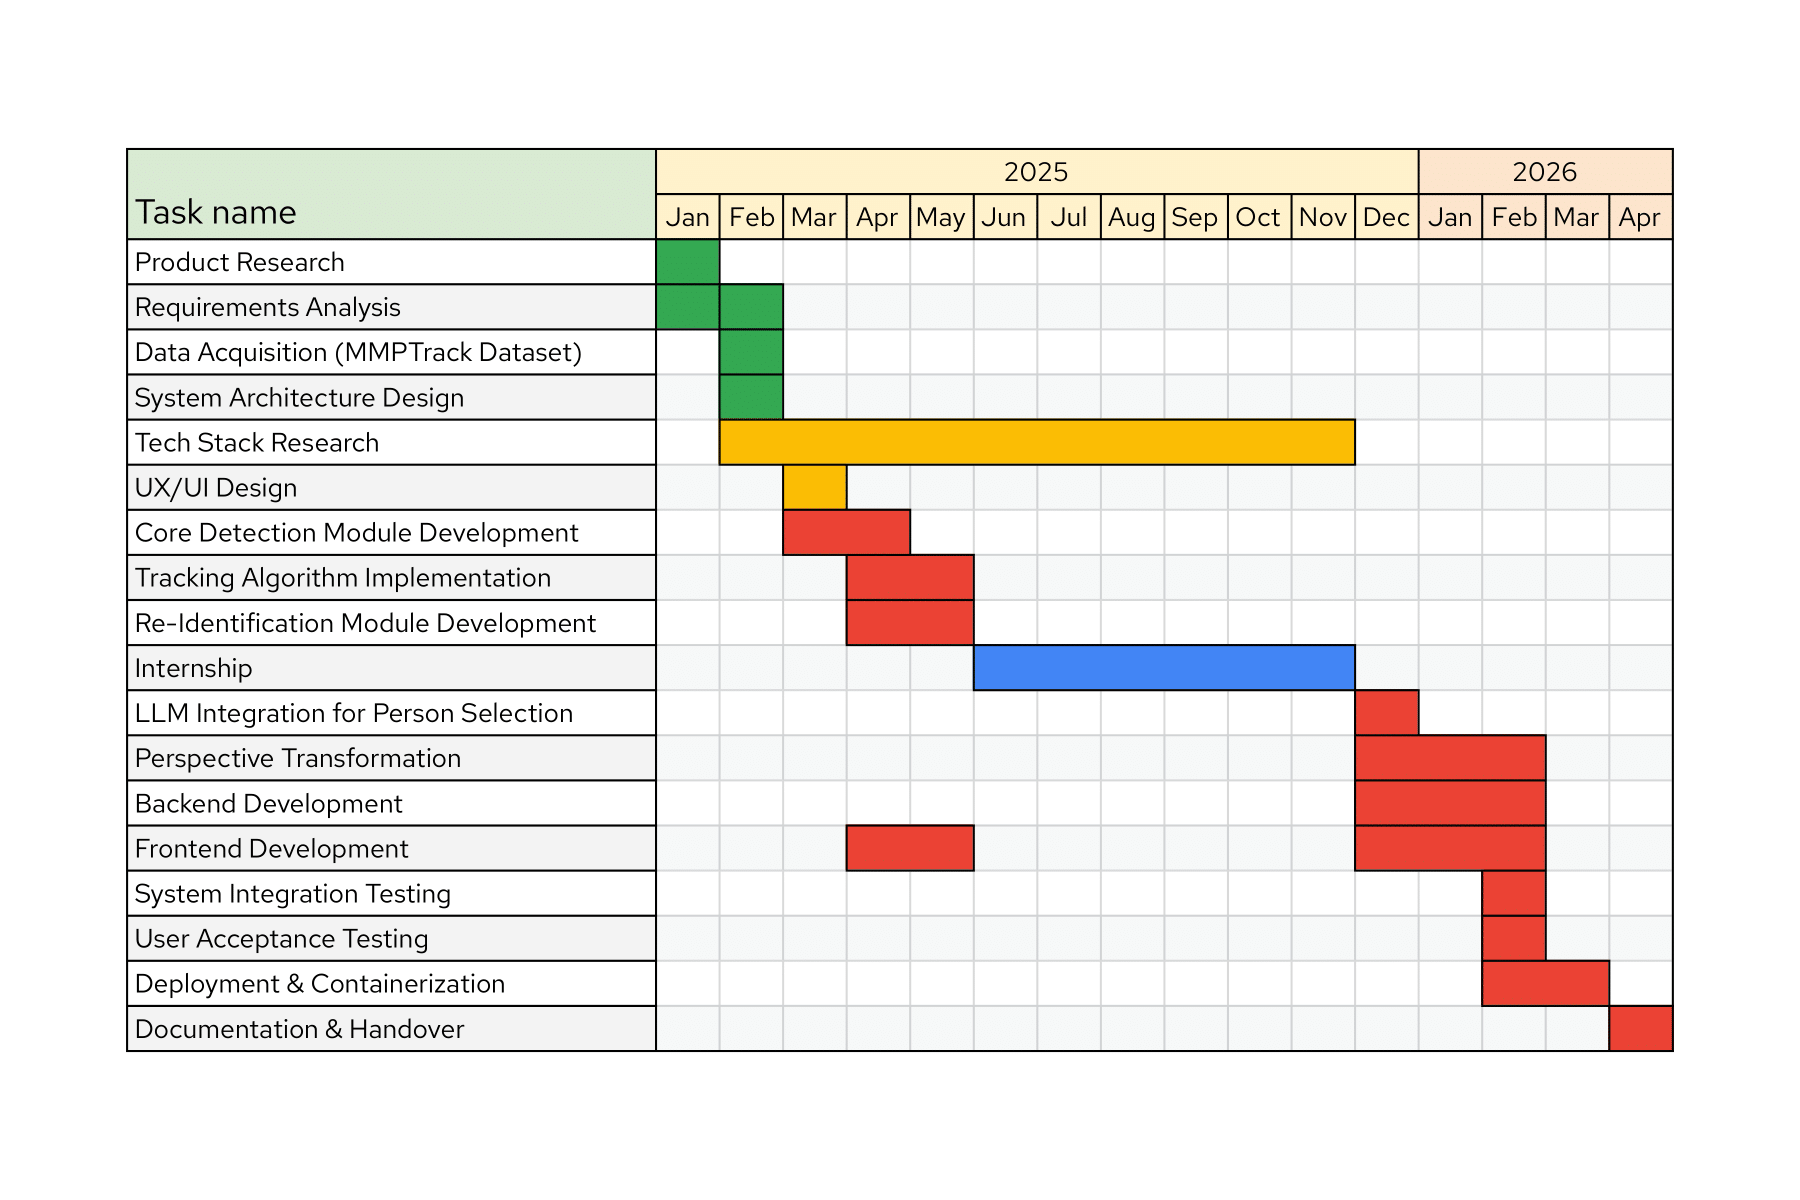
\includegraphics[width=\textwidth,height=\textheight,keepaspectratio]{jubjones/timeline.png}
    \caption{Timeline for Intelligent Multi-Camera Person Tracking System Project}
    \label{fig:timeline}
\end{figure}

As shown in figure \ref{fig:timeline}, it represents the timeline of the project.
The project began with system architecture design in January 2025, followed by the development of core detection
and tracking modules optimized for urban environments in February 2025. The re-identification and LLM integration components are scheduled for
completion by mid-March 2025.

System integration testing with actual urban camera networks will commence in late March 2025, with user acceptance testing planned for early April 2025.
The final deployment and handover are scheduled for completion by the end of April 2025, with ongoing support
and maintenance to follow.

\section{Terminology}
\label{section:terminology}

\begin{itemize}[leftmargin=40pt]
    \item \textbf{\textit{Object Detection}}---a computer vision technique that identifies and locates objects within digital images or video frames.
    \item \textbf{\textit{Re-Identification (Re-ID)}}---the process of matching individuals across different camera views by comparing appearance features extracted from images.
    \item \textbf{\textit{Multi-Target Multi-Camera Tracking (MTMCT)}}---the task of tracking multiple individuals across a network of cameras with non-overlapping fields of view.
    \item \textbf{\textit{Large Language Model (LLM)}}---an AI system trained on text data that enables natural language interactions for person description and filtering.
    \item \textbf{\textit{Perspective Transformation}}---a technique that converts observations from multiple camera views into a standardized coordinate system for unified spatial representation across an urban area.
    \item \textbf{\textit{Appearance Feature Embedding}}---a numerical representation of a person's visual characteristics that enables matching across different camera views despite viewing angle and lighting variations.
\end{itemize}